\graphicspath{ {Background/Images/} }


\chapter{Generalized Word2Vec}
\label{cha:background}

\section{Introduction}
In this chapter we introduce important concepts which are needed to understand our approach. These concepts can be used to solve problems described in chapter \ref{cha:context}. \\

We start with explaining some background knowledge in section \ref{sec:bk} such as time series and machine learning. We focus on basic concepts from machine learning and then focus more on neural networks. The main part to understand our approach is the introduction of Word2vec in section \ref{sec:word2vec}. This is then used to introduce Deepwalk as an extension on Word2Vec in section \ref{sec:deepwalk}. \\

After introducing those concepts, we explain our generalized Word2Vec approaches in section \ref{sec:gw2v}.


\section{Background Knowledge}
\label{sec:bk}

	\subsection{Time Series Analysis}
A time series consists of data points over a certain time period. We refer to this as a sequence of states. Where a state represents a data point and can differ from a single value to more complex representations like pictures. \\
The domain of time series analysis handles around extracting information or relations from a time series. It can have different goals like forecasting, classification, or exploratory. \\

A medical history of a patient can be seen as a time series, namely a sequence of EHRs. This means that methods which are applied on time series, are also applicable on medical data to find patterns.

	\subsection{Machine Learning}
Machine learning is a data driven approach with as goal to build a model which can be	used to make predictions or decisions. Note that this model can be used to predict outcomes of time series. This task is done by algorithms which are able to learn models based on examples given by the designer. Based on the examples, machine learning aims to tackle $3$ types of problems, namely supervised learning, unsupervised learning, and reinforcement learning. \\
Supervised learning is concerned with the learning task where there are examples given with their corresponding label. Unsupervised learning is similar to supervised learning only no labels are given. We won't go into reinforcement learning. \\
We can also classify the problems according to the desired output of our model. Those main tasks consist of classification, regression, and clustering. \\
	
We mention some used methods in the field of machine learning. These are used in above mentioned problems. \\
In the field of classification neural networks are used to achieve state of the art results. For regression, support vector machines can be used. One of the most popular methods for clustering is K-means. 

	\subsection{K-nearest Neighbors}
	\label{sec:knn}
	
The k-Nearest Neighbors (knn) algorithm is a simple machine learning algorithm \cite{knn:article}. It will be used in our generalized Word2Vec approach. \\
When you are in a supervised context, you have several instances with labels. When you retrieve a new instance, you want to predict its label. Based on a defined similarity measure (ex. Euclidean distance), you can look for the $k$ nearest labeled instances distanced to the new instance. From those, you pick the most common label in the pool of the $k$ nearest instances. This label becomes your predicted label for the new instance.
	
	
	\subsection{K-dimensional Tree}
	\label{sec:kdtree}
	
A naive way to calculate the nearest neighbors for a new element in a vector space, is by comparing all members with the new element and keep track of those distances. \\
A more efficient way is to use a k-dimensional tree (kd tree) \cite{kdtree:article}. In this section we explain the workings of this approach in more detail \cite{kdtreeIntro:atricle}. \\

A kd tree is a way of storing k-dimensional points. It is a binary tree where each node represents an element in the vector space. The node also contains information on how the tree is split up. It keeps track of the plane it is split on and the left and right sub tree. In figure \ref{fig:kdtreeSplit} you can see an example on how a simple kd tree is made and how it splits up the x,y plane. In the upper figure, the splitting plane is not mentioned, it is the $y=5$ plane for the $[2,5]$ and $x=3$ for $[3,8]$. \\
	
\begin{figure}[!htb]
	\centering
	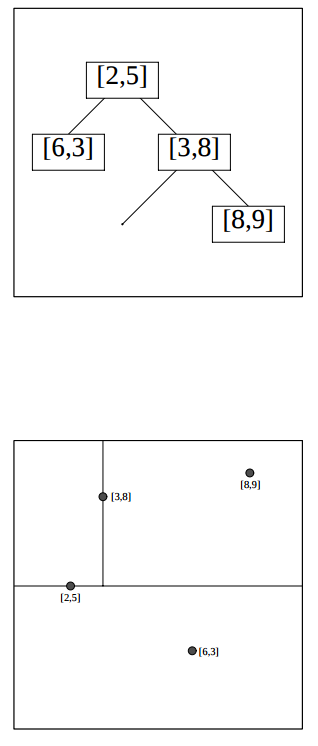
\includegraphics[width=0.4\textwidth]{kdtreeSplit.png}
	\caption{Representation on how a binary kd tree splits up the plane  \cite{kdtreeIntro:atricle}}
	\label{fig:kdtreeSplit}
\end{figure}

Now that we can construct the kd tree, we can use it to find the nearest neighbor for a certain input point. \\
We start with root node and recursively go down the kd tree. At each node it goes to the left or right depending on if the input is lesser or greater than the current nodes value on the splitting plane. Once it reaches a leaf node, it marks this node as the current nearest neighbor. \\
The algorithm unwinds the recursion of the tree, performing the following steps at each node:
\begin{itemize}

\item If the current node is closer than the current best, then it becomes the current best.
\item It checks if it is possible whether there is the possibility of closer points on the other side of the splitting plane. It makes a hypersphere around the current node with a radius equal to the current nearest distance. 
\begin{itemize}
\item If the hypersphere crosses the splitting plane, there could be a closer point on the other side. This means the algorithm will move down the other branch of the current node.
\item If the hypersphere does not cross the splitting plane, the whole other branch can be skipped.
\end{itemize}
\end{itemize}

This algorithm is easily extended to find the k-nearest neighbors by keeping track of the k current bests.
	
	\subsection{Neural Networks}
	
A neural network is a machine learning approach based on biological neural networks. It can be used to find patterns and do predictions on time series. Those time series can be medical data.


		\subsubsection{Perceptron}

The basic component of a neural network is a perceptron \cite{perceptron:article}. A perceptron takes multiple binary inputs and has a single binary output (see figure \ref{fig:perceptron}). Each input has a corresponding real numbered weight $w_j$. The output is decided on the following equation: \\

\begin{equation} 
output =
  \begin{cases}
    0       	& \quad \text{if } \sum_j w_jx_j \leq \text{ threshold}\\
    1  		& \quad \text{if } \text{if } \sum_j w_jx_j > \text{ threshold}\\
  \end{cases}
\end{equation}
	
\begin{figure}[!htb]
	\centering
	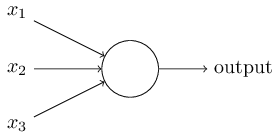
\includegraphics[width=0.4\textwidth]{perceptron.png}
	\caption{Simple presentation of a perceptron \cite{NNintro:online}}
	\label{fig:perceptron}
\end{figure}

We can build a network by connecting multiple perceptrons (see figure \ref{fig:multiplePerceptrons}). By building these networks, more complex decisions can be made. The reason for this, is that once there are atleast $3$ layers of perceptrons (and non-linear activation functions), the network can find non-linear relations between the input and output \cite{nnNL:article}. \\

\begin{figure}[!htb]
	\centering
	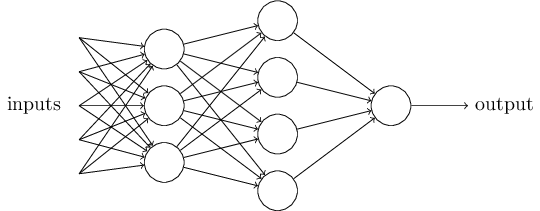
\includegraphics[width=0.8\textwidth]{multiplePerceptrons.png}
	\caption{More complex network made by connecting multiple perceptrons \cite{NNintro:online}}
	\label{fig:multiplePerceptrons}
\end{figure}

Now we have seen how a general network is constructed, we look at some vocabulary. \\
In figure \ref{fig:networkArch}, we see a four-layer network. As mentioned on the figure, we call the first layer the input layer, the last layer the output layer, and the layers in between are called hidden layers. Sometimes a multiple layer network is referred to as multilayer perceptrons or MLP. 

\begin{figure}[!htb]
	\centering
	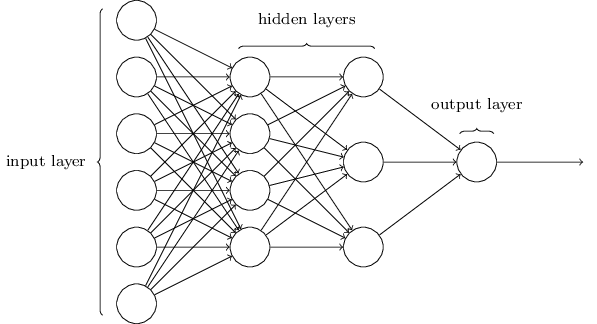
\includegraphics[width=0.8\textwidth]{networkArchitecture.png}
	\caption{General vocabulary of a multilayer network \cite{NNintro:online}}
	\label{fig:networkArch}
\end{figure} 		


		\subsubsection{Training a network}
		
To train a neural network, we input an example with a known label. The network will calculate a certain output based on the current weights (forward pass). When this output is incorrect, it should be possible to adjust the weights with as effect that the network now has as output the correct label (backward pass). Note that the change in weights, should only effect the output by a small bit (see figure \ref{fig:smallChange}). The reason for this is that otherwise all the previous inputs could now be labeled incorrectly. So, the concept of training a neural network means, adjusting the weights in a way that the behavior of the network doesn't change completely on the previous seen examples but that the current examples is labeled correctly. \\

\begin{figure}[!htb]
	\centering
	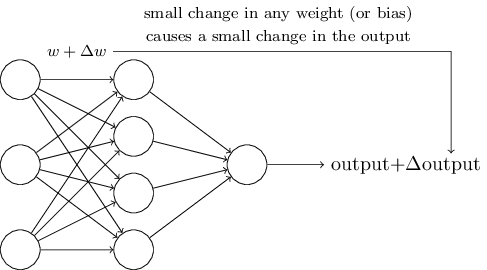
\includegraphics[width=0.8\textwidth]{smallChange.png}
	\caption{Small change on the weights, only has a small impact on the output \cite{NNintro:online}}
	\label{fig:smallChange}
\end{figure} 

To achieve this effect, we change our above explained perceptrons to sigmoid neurons. A sigmoid neuron has the same basics as a perceptron. It still has inputs but now it also has a bias $b$. The inputs still have weights but the weights can now range between $0$ and $1$. The output is now calculate with $\sigma(w*x+b)$ where $\sigma$ is the sigmoid function. This results in the following formula: 

\begin{equation} 
\frac{1}{1+exp(-\sum_j w_jx_j-b)}
\end{equation}

\noindent The sigmoid function makes it possible to calculate the gradient and makes the output a linear combination of $\Delta w_j$ and $\Delta b$ as $\Delta output$ is approximated by 

\begin{equation} 
\Delta output \approx \sum_j \frac{\partial output}{\partial w_j}\Delta w_j + \frac{\partial output}{\partial b}\Delta b
\end{equation}

\noindent Because of the linearity, it is now easier to choose changes for the weights and biases to achieve a correct output. By adjusting the weights, we will train our network to achieve a higher accuracy on the seen examples.
		
	\subsection{Backpropagation}
	
Backpropagation is an algorithm which is used to train neural networks \cite{bp:article}. It calculates the gradient of a chosen cost function with respect to the individual weights. Based on the gradient, the weights are updated and the cost function is minimized.

		\subsubsection{Terminology}
		
We use $w^l_{jk}$ to denote the weight corresponding to the connection between the $k^{th}$ node in the $(l-1)^{th}$ layer and the $j^{th}$ node in the $l^{th}$ layer. We use $b^l_j$ for the bias of the $j^{th}$ node in the $l^{th}$ layer and $a^l_j$ for the activation of the $j^{th}$ node in the $l^{th}$ layer. See figure \ref{fig:termNN}. \\

\begin{figure}[!htb]
	\centering
	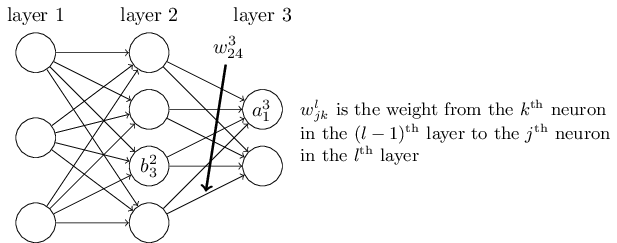
\includegraphics[width=0.8\textwidth]{termNN.png}
	\caption{Visual representation of the terminology for a neural network \cite{NNintro:online}}
	\label{fig:termNN}
\end{figure} 

\noindent We can now convert this notation to a vector representation. We remove the indexes for the node numbers which results in the following:

\begin{equation} 
a^l = \sigma (w^la^{l-1}+b^l)
\end{equation}

		\subsubsection{Cost function}
		
As mentioned before, backpropagation has as goal to calculate the partial derivatives of the cost function $C$ with respect to each weight and bias. \\
The cost function has to fulfill certain criteria. The first one is that it needs to be possible to write it as a summation over cost functions for individual training examples. Secondly, it needs to be derivable. And lastly, the cost function is a function of the activations of the last layer. 


		\subsubsection{Fundamental equations}

Backpropagation has 4 equations. They allow us to calculate the error for each node and adjust the weights based on the gradient descent. \\

First we calculate the error of each node which is based on how much the cost function is influenced by each of its activation and on how much the activation function is influenced by $z_j^L$:

\begin{equation} 
\delta^L_j = \frac{\partial C}{\partial a^L_j} \sigma'(z_j^L)
\text{ with }
z_j^L = \sum_k w^L_{jk}a^{L-1}_k+b^L_j
\end{equation}

\noindent This can be written as a neat vector equation:

\begin{equation} 
\delta^L = (a^L-y) \circ \sigma'(z_j^L)
\end{equation}

\noindent The next equation explains why the algorithm is called backpropagation. The equation calculates each layers error vector based on the layer after it, it propagates the error back over the layers:

\begin{equation} 
\delta^l = ((w^{l+1})^T\delta^{l+1}) \circ \sigma'(z_j^L)
\end{equation}

\noindent With those 2 equations we calculate the error in each layer of the neural network. Those errors can be used to calculate the derivatives of the cost function with respect to the weights and the biases:

\begin{equation} 
\frac{\partial C}{\partial w^l_{jk}} = a^{l-1}_k \delta^l_j.
\end{equation}

\begin{equation} 
\frac{\partial C}{\partial b^l_j} = \delta^l_j.
\end{equation}

\noindent When the derivatives are calculated, we can apply the gradient descent and update the weights and biases accordingly. This process represents the learning of a neural network.


\section{Word2Vec}
\label{sec:word2vec}

\subsection{Motivation}

We will explain Word2Vec in this section. It is explained from a linguistic point of view. This explanation is needed to introduce our generalized Word2Vec approach which can be applied to medical data. \\

In natural language processing tasks, a good representation of words helps learning algorithms perform better. A representation is learned which maps words to vectors in a low-dimensional space compared to the vocabulary size. In this representation, we try to map context-similar words close to each other in the new vector space. The new representation is sometimes also called a 'word embedding'. \\
We could say in an informal way: a linguistic background is made which the learning algorithm can use. 


\subsection{Skip-gram}

There are two main models used for Word2Vec \cite{w2vOriginal:article}, namely Continuous Bag-of-Words (CBOW) and the Skip-Gram model. \\
The first one tries to predict a word based on a given context (ex. predict Paris when capital France is given). And the second one does the inverse of this approach \cite{w2vModels:article}. Empirical results have shown that the Skip-Gram model tends to do better on larger datasets \cite{w2vReason1:online} and gives a better representation for infrequent words \cite{w2vArchive:online}. In medical data there are often infrequent cases which are important. For those reasons, we choose to go further with the Skip-Gram model. \\

So one way of learning a Word2Vec representation of a corpus $Text$, is by using the Skip-Gram model. \\
Based on given words $w$ and their contexts $c$, we set the parameter $\theta$ of $p(c|w;\theta)$ to maximize:

\begin{equation} 
\arg \max_{\theta} \prod_{(w,c \in D)} p(c|w;\theta)
\end{equation}

\noindent with $D$ the set of all word and context pairs we extract from the corpus.\\
Here we also note that $p(c|w)$ is indeed the chance of a context appearing after seeing a specific word as mentioned before.

\subsubsection{Finding word-context pairs}

Given a sequence of words, we define their context based on n-grams \cite{w2vNgram:article}. In figure \ref{fig:ngram}, n-grams are explained on the sentence "This is a sentence". 

\begin{figure}[htbp]
	\centering
	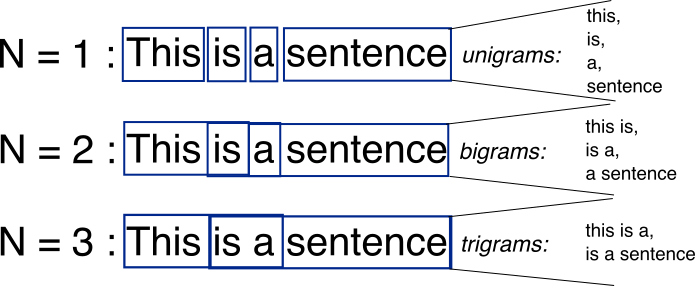
\includegraphics[width=0.8\textwidth]{ngram.png}
	\caption{Explanation of n-gram \cite{w2vNgram:online}}
	\label{fig:ngram}
\end{figure} 

For the Skip-gram model, we define the context of a word $w_t$ as $w_{t+j}$ with $j$ between $-c$ and $c$. A larger $c$ typically results in more specific contexts for training examples and thus can lead to a higher accuracy if there is enough data to back this up. Because if there are not enough cases handling those specific contexts, the correlation between the word and his context is less statistically significant.


\subsubsection{Parameterization}

We start with rewriting the conditional probability using soft-max:

\begin{equation} 
p(c|w;\theta) = \frac{e^{v_x*v_w}}{\sum_{c' \in C}e^{v_{c'}*v_w}}
\end{equation}

\noindent where $v_c$ and $v_w$ are vector representations for $c$ and $w$, and $C$ is the set of all available contexts. This means that the parameters $\theta$ are $v_{c_i}$ and $v_{w_i}$. Computing the optimal parameters is very expensive because you need to calculate this over all contexts $c'$. We also switch from product to sum by taking the logs:

\begin{equation} 
\arg \max_{\theta} \sum_{(w,c) \in D} \log p(c|w;\theta) = \sum_{(w,c) \in D} (\log e^{v_c * v_w} - \log \sum_{c'} e^{v_{c'}*v_w})
\end{equation}

\subsection{Negative Sampling}

To compute the vectors using the Skip-gram model more efficiently, we introduce negative sampling \cite{w2vExplained:article}. \\
Instead of calculating $\sum_{c' \in C}e^{v_{c'}*v_w}$ over all contexts, we make a set $D'$ which consists of randomly sampled word-context pairs. With this new set, we remove the costly term $\sum_{c' \in C}e^{v_{c'}*v_w}$ and replace it with $\sum_{(w,c) \in D'}e^{v_{c'}*v_w}$. \\

In a less formal way: we are not making sure that if words appear in the same context, their vectors are more similar than all the other word vectors, but only more similar than several vectors chosen randomly. This makes the Skip-gram model usable in terms of computation.


\subsection{Neural Networks}

When the Word2Vec algorithm is trained using the Skip-gram model, one will have a lookup table. This table contains the mapping of words to their vector representation. This lookup table can be found by training a 2-layer neural network with as cost function the function described in the previous section. The training can be done with backpropagation for example. \\
The trained 2-layer neural network can be placed in front of another neural network \cite{w2vNN:online}. It will convert the words to their vector representation and feed it into the next neural network. It is empirically shown that this can improve the results of the neural network by putting the lookup table in front of it. As mentioned before, in a way, you offer background knowledge to the neural network.

\section{DeepWalk}
\label{sec:deepwalk}

DeepWalk is an approach where graph structured data is transformed into sequences of vertices \cite{deepwalkMain:article}. Word2Vec is then applied on those sequences to learn a good vector representation for the vertices. We can say that it is an extension on the Word2Vec approach. \\

In figure \ref{fig:dwAlgo}, we see an overview of the DeepWalk algorithm. It exist of two parts. \\
First a random walk generator. For each vertex $v_i$ of the graph $G$, it will generate a random walk of length $t$. It will do this $\gamma$ times but the order to which the vertices are traversed, is randomly ordered each pass. With those walks, a sequence of vertices is generated. \\
Secondly, those vertices are used for Word2Vec. This process is explained in section \ref{sec:word2vec}.

\begin{figure}[!htb]
	\centering
	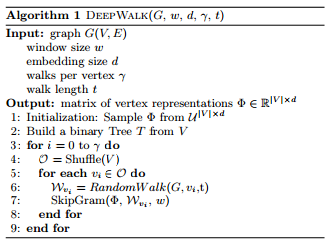
\includegraphics[width=0.7\textwidth]{dwAlgo.png}
	\caption{Overview of the DeepWalk algorithm \cite{deepwalkMain:article}}
	\label{fig:dwAlgo}
\end{figure} 

\section{Generalized Word2Vec Approaches}
\label{sec:gw2v}

In this section we explain our approach on how to find patterns in EHRs. For this, we use generalized Word2Vec approaches to learn disease embeddings. 

\subsection{Data representation}

Before we can start with explaining how Word2Vec can be applied on EHR data, we start with introducing our data representation. \\
The medical history of a patient is a time series of EHRs. On certain timestamps, an EHR is available containing the medical state of that patient. We call this EHR the vector $m^p_t$, with $p$ a patient number and $t$ a timestamp. This means that each patient has a sequence of vectors $s^p = m^p_t, m^p_{t+1}, m^p_{t+3}, \ldots$ Each vector $m^p_t$ contains certain values depending on the EHR. It can contain values of the timestamp, demographics, blood pressure, diagnoses, and others. 

\subsection{Generalized Word2Vec}

As explained in section \ref{sec:word2vec}, Word2Vec is applied on a large text corpus containing a large amount of sentences. After applying this method, an embedding is found that represents words in a new vector space. In this vector space the relationship between words is shown by the distance of the words from each other. \\

A large medical dataset containing EHRs from different patients, can be seen as a large text corpus. It contains patients, each having a sequence $s^p$, which is equivalent to one sentence. All the different patients sequences, make the whole dataset similar to how sentences make a text corpus. Each vector $m^p_t$ is removed from its link to the patient and his timestamp to make it not unique anymore, we call this vector $m$. This is to make the link to words. Different sentences can contain the same words, similar to how the vectors $m$ are in the different sequences. \\

With those links, it is possible to apply Word2Vec not only to simple objects like words, but also on more abstract objects like vectors. We call this a generalized Word2Vec approach. From this, we can learn an embedding for the vectors $m$ in the new vector space. In this new vector space, the relationships between the vectors $m$ are found based on their occurrences with others in the sequences. \\

We can now apply Word2Vec to medical data. The vector $m$ is an EHR and by applying the generalized Word2Vec method, we find an embedding for the vectors $m$. The result is a disease embedding which projects the EHR data to a new vector space and projects EHRs which have a close relationship to each other, close to each other in the new vector space.


\subsection{K-Nearest Neighbors Word2Vec}

A problem with using an embedding which is found on a certain dataset, is that it is possible that certain instances are not present in the dataset. In the case of a complete new instance, a Word2Vec model cannot find a representation for this instance. As we are working in the context of a generalized Word2Vec approach, where instances are represented by complex objects like vectors, the chances of this happening increases. It increases because there are a lot more possible combination of vectors possible than there are words in a dictionary for example. \\

Therefore we introduce a K-Nearest Word2Vec approach. As we are working with more abstract objects, namely vectors, we can extend our generalized Word2Vec approach with a knn feature (see section \ref{sec:knn}). After the training of a Word2Vec model, we have learned a lookup table which maps a known vector $v_{old}$ to his new vector representation $v_{new}$. When a not-yet-seen vector $v_{unknown}$ needs to be mapped to his $v_{new}$, a normal Word2Vec is not capable of this. \\
In our approach, we find the k-nearest neighbors of the $v_{unknown}$ from the old representations $v_{old}$ in the lookup table. We then take the new representations of the knn, and combine them using a weighted average to estimate the new representation $v_{new}$ for $v_{unknown}$. This way our approach is capable of handling complete new instances. \\

In short: we look for the knn of the $v_{unknown}$ from all the known vectors in the lookup table in their original representation $v_{old}$. Based on the found knn, we take an weighted average of the old representations $v_{old}$. This weighted average is the $v_{new}$ for the $v_{unknown}$.

\subsection{Generalized Deepwalk}

Deepwalk itself is hard to apply on EHR data as it starts from a graph structure. It however provides an extra Word2Vec approach which can be generalized to more abstract objects like vectors. \\

One application of Deepwalk is the need for less data to achieve a good Word2Vec model. When the EHR dataset becomes very large, it would take a considerable amount of time to train a Word2Vec model. Therefore it would be interesting to transform the EHR data into a weighted graph structure. The weights are based on the frequency of diagnoses following each other in all the sequences. \\
After the graph transformation, the amount of weighted random walks can be limited to create a smaller set of sequences based on the original dataset. Those sequences can be used to train a Word2Vec model faster as there is fewer data. The same logic from the previous two sections is applicable to generalize DeepWalk from words to more abstract objects.


\section{Conclusion}
In this chapter we talked about general machine learning concepts and focused on Word2Vec. We conclude that Word2Vec is used to find good representation of words based on their context. It also causes that similar words will be close to each other in this new representation. \\

With the concepts explained, we introduced our approaches. We extended Word2Vec so that it can handle more abstract objects than words, namely vectors representing an EHR. We also extended Word2Vec to find a representation for a new instance based on knn. Also DeepWalk is generalized to more abstract objects.



%%% Local Variables: 
%%% mode: latex
%%% TeX-master: "thesis"
%%% End: 
